\documentclass[a4paper, 10pt]{article}
\usepackage{pgf}
\usepackage{eurosym}
\usepackage{graphicx}
\usepackage{wasysym}
\usepackage{hyperref}
\usepackage{listings}
\usepackage{pxfonts}
\usepackage{verbatim}
\usepackage{color}
\usepackage{xcolor}
\usepackage{wrapfig}
\usepackage{enumitem}
\usepackage{booktabs}
\usepackage{tabularx}

\hypersetup{
    bookmarks=true,         % show bookmarks bar?
    unicode=true,          % non-Latin characters in Acrobat’s bookmarks
    pdftoolbar=true,        % show Acrobat’s toolbar?
    pdfmenubar=true,        % show Acrobat’s menu?
    pdffitwindow=true,     % window fit to page when opened
    pdftitle={Assignment 2},    % title
    pdfauthor={Paul Vesey},     % author
    pdfsubject={Construction Project Management},   % subject of the document
    pdfcreator={},   % creator of the document
    pdfproducer={xelatex}, % producer of the document
    pdfkeywords={'Project Management' }, % list of keywords
    pdfnewwindow=true,      % links in new PDF window
    colorlinks=true,       % false: boxed links; true: colored links
    linkcolor=violet,          % color of internal links (change box color with linkbordercolor)
    citecolor=magenta,        % color of links to bibliography
    filecolor=red,      % color of file links
    urlcolor=blue           % color of external links
}

\setlength\parindent{0pt}
\begin{document}

\lstset{language=HTML,
				basicstyle=\small,
				breaklines=true,
        numbers=left,
        numberstyle=\tiny,
        showstringspaces=false,
        aboveskip=-20pt,
        frame=leftline
        }
				
\begin{table}%
	\begin{minipage}{0.4\textwidth}%
			
\includegraphics[width=1\textwidth]{./img/LITlogo.jpg}
	\end{minipage}
	\qquad
	\centering
	\parbox{0.4\textwidth}{
		\begin{large}			
			\begin{tabular}{| r | l |} \hline
				Subject: & \textbf{Construction Project Management}\\
				Course: & \textbf{CPM Special Purpose Award}\\	
				Session: & \textbf{Spring 2020}\\
				Lecturer: & \textbf{Paul Vesey \footnotesize{BEng, MIE, HDip}}\\
				\hline
			\end{tabular}
		\end{large}			
	}
\end{table}
\vspace{0.25cm}	
	

\part*{Assignment 3 (35\%)- Project Management Initiating and Planning Documents}


\begin{tabularx}{\textwidth}{ |X|X| }
	\hline
	\textbf{Issue Date:} & 16$^{th}$ March 2021\\
	\hline 
	\textbf{Submission Date:}  & 30$^{th}$ April 2021\\
	\hline
\end{tabularx}

\section*{Introduction}

This is an individual project.  You are encouraged to discuss your project with your peers, however all work submitted must be your own, with attribution where appropriate.\\

In this assignment you are required to create a detailed project plan for a construction project of your choice.  The project plan should include the traditional project management documents as well as a Post Contract Award BIM Execution Plan.  You are free to use the documentation pack used for Assignment 2.\\

The key deliverables for this prohect are:

\begin{enumerate}
	\item Detailed Project Management Plan 
	\item Post Contract BIM Execution Plan
\end{enumerate}


\section*{Scenario}

Select a project with which you are familiar. The project must be a construction related project where BIM was or could be deployed.  The project must have at least 20 tasks and a maximum of 30.\\

Develop the following items as detailed below. Descriptions of items 1 to 10 are available in the lecture notes, and are based on PMI's Project Management Body of Knowledge\\

You are advised to use the RIAI Template for Item 11, the Post Contract BIM Execution Plan, available on OneNote.\\

The objective of this assignment is to produce a comprehensive project plan. The text of the document should clearly show how the various aspects of the project are going to be managed and controlled. You are encouraged to use standard templates and methodologies.  Standard Templates and Methodologies should be correctly attributed.\\

Your final document should be of professional standard in terms of content, layout and completeness. In essence, the completed document should be suitable for presentation to a prospective client.\\

The Reflective Statement should detail your learning experience while undertaking this coursework and your opinion on its relevance to the subject, etc.\\

You are encouraged to use Microsoft Project, Autodesk Revit, BIM 360 and other applications as appropriate.\\

This is a practical assignment. Your project management document should fully based on the practical implementation of project management theory.\\


\section*{Late Submission}
Failure to submit your assignment on or before the date and time indicated on MS Teams will result in a penalty of 5\% per day or part thereof.


\newpage

\section*{Marking Scheme}
\begin{table}[ht]
	\centering
	\begin{tabular}{|c|l|c|c|}
		\hline
		\textbf{Item} & \textbf{Description} & \textbf{Maximum Required} & \textbf{Marks \%} \\
		\hline
		\hline

		1  & Project Scope Statement &  2 pages  & 10\% \\
		\hline

		2  & Work Breakdown Structure &  30 elements  & 5\% \\
		\hline

		3  & Resource Breakdown Structure &  15 elements  & 5\% \\
		\hline

		4  & RACI Responsibility Assignment Matrix &  A3 Diagram  & 5\% \\
		\hline

		5  & Network Diagram and Gantt Charts &  A3 Diagrams  & 5\% \\
		\hline

		6  & Risk Management Plan & 2 pages  & 10\% \\
   			&	- Methodology  & & \\
   			&	- Timing of Risk Events  & & \\
   			&	- Risk Register  & & \\
		\hline
		
		7  & Cost Control Plan &  2 pages  & 5\% \\
   			&	- Total value of contract  & & \\
   			&	- Proportion to contractor  & & \\
   			&	- Proportion subcontracted   & & \\
   			&	- Methodology  & & \\
   			&	- Project Cash Flow Profile  & & \\
		\hline

		8  & Communications Plan &  2 pages  & 5\% \\
   			&	- Stakeholder Identification Method  & & \\
   			&	- Information Distribution Plan  & & \\
   			&	- Performance Report Requirements  & & \\
		\hline

		9  & Human Resource Plan &  1 page  & 10\% \\
   			&	- Project Team Acquisition  & & \\
   			&	- Release Criteria  & & \\
		\hline

		10  & Procurement Management Plan &  1 page  & 5\% \\
   			&	- Seller Selection Procedure  & & \\
   			&	- Contract Types  & & \\
		\hline

		11  & Post Contract BIM Execution Plan &  see template  & 30\% \\
		\hline
		12  & Reflective Statement &  1 page  & 5\% \\
		
		
		\hline
		\hline
        & & \textbf{Total} & \textbf{100\%} \\
		\hline
	
	\end{tabular}
	\caption{Table }
	\label{tab:AM}
\end{table}


\newpage

\section*{Reflective Practice Framework}

There are numerous reflective practice frameworks in common use.  The diagram below depicts the Gibbs Reflective Cycle.  You are free to use any methodology.


\begin{figure}[h!]
	\centering
	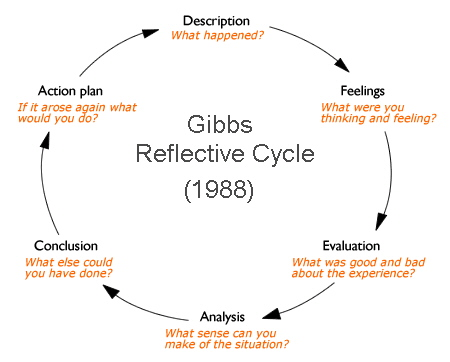
\includegraphics[width=1.0\linewidth]{img/gibbs-diagram}
	\caption{Gibbs Reflective Cycle}
	\label{fig:gibbs-diagram}
\end{figure}




\end{document}